\iffalse
\documentclass[journal,10pt,twocolumn]{article}
\usepackage[margin=0.5in]{geometry}
\usepackage[cmex10]{amsmath}
\usepackage{array}
\usepackage{booktabs}

% The preceding line is only needed to identify funding in the first footnote. If that is unneeded, please comment it out.
\usepackage{cite}
\usepackage{amsmath,amssymb,amsfonts}
\usepackage{graphicx}
\usepackage{textcomp}
\usepackage{xcolor}
\usepackage{graphicx}
\graphicspath{{./fig}}{}
\def\BibTeX{{\rm B\kern-.05em{\sc i\kern-.025em b}\kern-.08em
    T\kern-.1667em\lower.7ex\hbox{E}\kern-.125emX}}

\usepackage{tikz}
\usetikzlibrary{shapes.geometric}
\usetikzlibrary{shapes.geometric,angles,quotes}


\begin{document}



\newtheorem{theorem}{Theorem}[section]
\newtheorem{problem}{Problem}
\newtheorem{proposition}{Proposition}[section]
\newtheorem{lemma}{Lemma}[section]
\newtheorem{corollary}[theorem]{Corollary}
\newtheorem{example}{Example}[section]
\newtheorem{definition}[problem]{Definition}
%\newtheorem{thm}{Theorem}[section] 
%\newtheorem{defn}[thm]{Definition}
%\newtheorem{algorithm}{Algorithm}[section]
%\newtheorem{cor}{Corollary}
\newcommand{\BEQA}{\begin{eqnarray}}
\newcommand{\EEQA}{\end{eqnarray}}
\newcommand{\define}{\stackrel{\triangle}{=}}
\newcommand*\circled[1]{\tikz[baseline=(char.base)]{
    \node[shape=circle,draw,inner sep=2pt] (char) {#1};}}

\bibliographystyle{article}
%\bibliographystyle{ieeetr}


\providecommand{\mbf}{\mathbf}
\providecommand{\pr}[1]{\ensuremath{\Pr\left(#1\right)}}
\providecommand{\re}[1]{\ensuremath{\text{Re}\left(#1\right)}}
\providecommand{\im}[1]{\ensuremath{\text{Im}\left(#1\right)}}
\providecommand{\qfunc}[1]{\ensuremath{Q\left(#1\right)}}
\providecommand{\sbrak}[1]{\ensuremath{{}\left[#1\right]}}
\providecommand{\lsbrak}[1]{\ensuremath{{}\left[#1\right.}}
\providecommand{\rsbrak}[1]{\ensuremath{{}\left.#1\right]}}
\providecommand{\brak}[1]{\ensuremath{\left(#1\right)}}
\providecommand{\lbrak}[1]{\ensuremath{\left(#1\right.}}
\providecommand{\rbrak}[1]{\ensuremath{\left.#1\right)}}
\providecommand{\cbrak}[1]{\ensuremath{\left\{#1\right\}}}
\providecommand{\lcbrak}[1]{\ensuremath{\left\{#1\right.}}
\providecommand{\rcbrak}[1]{\ensuremath{\left.#1\right\}}}

\newcommand{\sgn}{\mathop{\mathrm{sgn}}}

%\providecommand{\hilbert}{\overset{\mathcal{H}}{ \rightleftharpoons}}
\providecommand{\system}{\overset{\mathcal{H}}{ \longleftrightarrow}}
	%\newcommand{\solution}[2]{\textbf{Solution:}{#1}}
\newcommand{\solution}{\noindent \textbf{Solution: }}
\newcommand{\cosec}{\,\text{cosec}\,}
\providecommand{\dec}[2]{\ensuremath{\overset{#1}{\underset{#2}{\gtrless}}}}
\newcommand{\myvec}[1]{\ensuremath{\begin{pmatrix}#1\end{pmatrix}}}
\newcommand{\mydet}[1]{\ensuremath{\begin{vmatrix}#1\end{vmatrix}}}
	\newcommand*{\permcomb}[4][0mu]{{{}^{#3}\mkern#1#2_{#4}}}
\newcommand*{\perm}[1][-3mu]{\permcomb[#1]{P}}
\newcommand*{\comb}[1][-1mu]{\permcomb[#1]{C}}

%\numberwithin{align}{section}
\numberwithin{align}{subsection}
%\numberwithin{problem}{section}
%\numberwithin{definition}{section}

\let\vec\mathbf




\title{
{Comparision of Angles and Sides of Trapezium\\
Using Matrices and lines}\\

\thanks{Meer Tabres Ali as an intern with FWC IIT Hyderabad. *The author is with the Department of Electrical Engineering, Indian Institute of Technology, Hyderabad 502285 India e-mail: gadepall@iith.ac.in. All content in this manual is released under GNU GPL. Free and open source.}
}
\author{Meer Tabres Ali and G V V Sharma}
\maketitle
\tableofcontents
\section{Problem statement}
\fi
$ABCD$ is trapezium in which $AB \parallel CD$ and $AD=BC$.
Show that, 
\begin{enumerate}
    \item $\angle A = \angle B$
    \item $\angle C = \angle D$
    \item Diagonal $AC$ = Diagonal $BD$
    \item $\triangle ABC  = \triangle BAD$
\end{enumerate}
\iffalse
\solution 
See Fig. 
		\ref{fig:9/8/1/12}.
	\begin{figure}[!h]
		\centering
 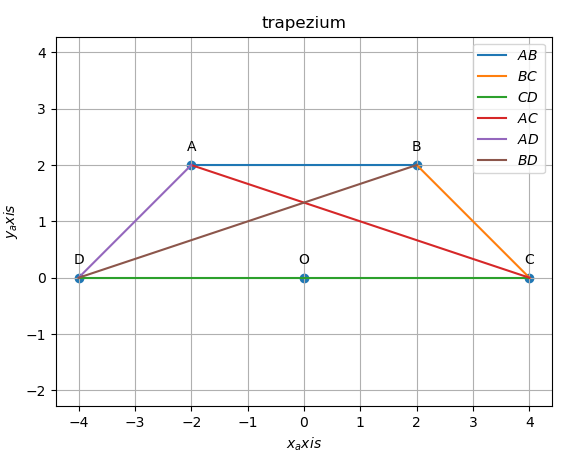
\includegraphics[width=\columnwidth]{chapters/9/8/1/12/figs/trapezium1.png}
		\caption{}
		\label{fig:9/8/1/12}
  	\end{figure}
For $\vec{e}_1$ defined in Appedix \ref{def:matrix-two},
    Let 
\begin{align}
	 \label{eq:9/8/1/12/cang}
		\begin{split}
	\vec{D} &= \vec{0}
	\\
	\vec{C}&= c\vec{e}_1
\\
	\vec{A}&= r\myvec{\cos D \\ \sin D}
\\
	\vec{B}&= \vec{C} +  r\myvec{-\cos C \\ \sin C}
		\end{split}
\end{align}
%
Thus, 
\begin{align}
	 \label{eq:9/8/1/12/cang/a}
	\cos \angle{BAD}
	&= \frac{(\vec{A}-\vec{B})^T(\vec{A}-\vec{D})}{\norm{\vec{A}-\vec{B}}\norm{\vec{A}-\vec{D}}}
	\\
\cos	\angle{CBA}
	 &= \frac{(\vec{B}-\vec{C})^T(\vec{B}-\vec{A})}{\norm{\vec{B}-\vec{C}}\norm{\vec{B}-\vec{A}}}
	 \label{eq:9/8/1/12/cang/b}
%
\end{align}
Substituting from 
	 \eqref{eq:9/8/1/12/cang},
\begin{align}
	 \label{eq:9/8/1/12/cang/abd}
	 (\vec{A}-\vec{B})^T(\vec{A}-\vec{D}) &= r\brak{r\myvec{\cos D+ \cos C  & \sin D - \sin C}-c\vec{e}_1^{\top}}\myvec{\cos D \\ \sin D}
	 \\
	&= r\brak{r\brak{1+ \cos \brak{C+D}  }-c\cos D }
\end{align}
Similarly, 
\begin{align}
	 \label{eq:9/8/1/12/cang/abc}
(\vec{B}-\vec{C})^T(\vec{B}-\vec{A})
	&= r\brak{-r\myvec{\cos D+ \cos C  & \sin D - \sin C}+c\vec{e}_1^{\top}}\myvec{-\cos C \\ \sin C}
	 \\
	&= r\brak{r\brak{1+ \cos \brak{C+D}  }-c\cos D }
\end{align}

	 \eqref{eq:9/8/1/12/cang},
\section{Considerations}
\vspace{0.2cm}
The input parameters are the lengths r, c and angle $\theta$. \\
\vspace{0.2cm}
{


\setlength\extrarowheight{2pt}
\begin{tabular}{|c|c|c|}
	\hline
	\textbf{Symbol}&\textbf{Value}&\textbf{Description}\\
	\hline
	$\vec{O}$ & \myvec{0\\0}
	&Origin\\
	\hline
	r&2.82& Distance of BC, AD\\
	\hline
	c&4&OC\\
	
	\hline
	$\vec{C}$ & \myvec{c \\ 0}

	&Point C on X axes
	\\
\hline
	$\theta$&45 \textdegree &$\angle$BOC\\
	\hline
\end{tabular}
}


\section{Plotting Trapezium}




\vspace{0.25cm}
Plot of Trapezium is shown in figure 1, where point O is origin and points A, B, C and D are the vertices of Trapezium.
\begin{figure}[h]

\caption{trapezium}
\label{fig:trapezium}
\end{figure}


\section{Solution}

\vspace{0.25cm}
\subsection{Finding Co-ordinates O, A, B, C and D}
\begin{flushleft}
Let O be the origin and its coordinates are\\
\vspace{0.25cm}

\center
\vspace{0.4cm}
$\vec{O}$ = \myvec{0\\0}
\endcenter{}
\vspace{0.25cm}
Let C be the point on X-axes and it is expressed as\\
\vspace{0.25cm}
\begin{align}
    \vec{C} = c
    \end{align}

\vspace{0.25cm}
\begin{flushleft}
Let D be the point on Negative X-axes and it will be the image of C,\\
\begin{center}
$\vec{D}$  = -c\\
\end{center}
\vspace{0.2cm}
Therefore, the coordinates of D are\\
\end{flushleft}


\vspace{0.25cm}
\begin{flushleft}
Let r be the distance between point B and C, then\\
\end{flushleft}

\vspace{0.25cm}
$|| \vec{B-C} || $ = r and $|| \vec{A-D} || $ = r\\
\vspace{0.25cm}
\begin{flushleft}
Let $\theta$ be the angle at BOC, then\\
\end{flushleft}
\vspace{0.25cm}
$\angle$BOC = $\theta$\\
\vspace{0.25cm}
\begin{flushleft}
According to the vector geometry formulaes, the vector B can be expresssed as\\
\end{flushleft}
\vspace{0.25cm}
\begin{align}
   \vec{B}= r \myvec{cos\theta \\ sin\theta}
\end{align}

\vspace{0.35cm}
\begin{flushleft}
From ABCD trapezium, \\
\end{flushleft}
\begin{center}
$\vec{A} =\vec{B}-  \vec{C}$\\
\end{center}

\center
\vspace{0.4cm}
= \myvec{rcos $$\theta$$ \\ rsin $$\theta$$} - \myvec{c \\ 0}
   
\endcenter{}
		= \myvec{-c+rcos $$ \theta$$ \\ rsin$$\theta$$}
	\\
\vspace{0.3cm}
\begin{flushleft}
From triangle ODA,
$\boldsymbol{OD+DA=OA}$, \\
\vspace{0.2cm} 
$\implies$ -c+rcos$\theta$ = -r cos $\theta$\\
\end{flushleft}
\vspace{0.35cm}
	= \myvec{-rcos $$ \theta$$ \\ rsin$$\theta$$} \\
\endcenter{}
	$\implies$ $\vec{A}$
	= r\myvec{-cos $$ \theta$$ \\ sin$$\theta$$} \\

Let c=4, r=2.82 and $\theta$=45 \textdegree \\

Then all the four coordinates will be, \\

\vspace{0.3cm}
$\vec{O}$=\myvec{0 \\ 0}, $\vec{A}$=\myvec{-2 \\ 2}, $\vec{B}$=\myvec{2 \\ 2}, $\vec{C}$=\myvec{4 \\ 0}, $\vec{D}$=\myvec{-4 \\ 0}
\\

\subsection{Calculation of Angles A and B}
\vspace{0.25cm}
To find angle $\angle$A:\\

\begin{center}
    

$\vec{A-D}$ = \myvec{-2 \\ 2} - \myvec{-4 \\ 0}
	= \myvec{2 \\ 2}

\begin{flushleft}
and \\
\end{flushleft}


$\vec{A-B}$ = \myvec{-2 \\ 2} -\myvec{2 \\ 2} = \myvec{-4 \\ 0}
	\\

\end{center}
\vspace{0.4cm}
\begin{align}
\angle BAD = arccos \vec{\frac{(A-D).(A-B)}{||A-D ||. ||A-B||}}
\end{align}
\vspace{0.4cm}
\begin{align}
\angle BAD = arccos \frac{(2 \hspace{0.32cm}  2)^T . (-4 \hspace{0.25cm}   0) } {\sqrt{2^2+2^2}.\sqrt{4^2+0}}
\end{align}

\begin{align}
= arccos \frac{-8 } {\sqrt{8}.\sqrt{16}} = arccos (-0.707) 
\end{align}
\begin{flushleft}
$\implies$   $\angle$ BAD = 135 \textdegree\\
\vspace{0.3cm}
$\implies$   $\angle$ A = 135 \textdegree
\end{flushleft}

\vspace{0.5cm}
\begin{flushleft}
To find angle $\angle$ B: \\
\end{flushleft}

\vspace{0.35cm}
$\vec{B-A}$ = \myvec{2 \\ 2}-\myvec{-2 \\ 2}
	= \myvec{4\\0}
and \\

$\vec{B-C}$ = \myvec{2 \\ 2} -\myvec{4\\0} = \myvec{-2 \\2} 
\vspace{0.25cm}	
\begin{align}
\angle BAD = arccos \vec {\frac{(A-D).(A-B)}{||A-D||.||A-B||}}
\end{align}

\begin{align}
\angle BAD = arccos \frac{(4, 0)^T .(-2, 2)}{\sqrt{4^2}.\sqrt{2^2+2^2} }
\end{align}

\begin{align}
= arccos \frac{-8 } {\sqrt{16}.\sqrt{8}} =arccos (-0.707)
\end{align}

\begin{flushleft}
$\implies$   $\angle$ ABC = 135 \textdegree\\
\vspace{0.3cm}
$\implies$   $\angle$ B = 135 \textdegree
\\
\vspace{0.3cm}
Therefore $\angle A$ = $\angle B$
\end{flushleft}

\subsection{Calculation of Angles C and D}
\vspace{0.25cm}

To find angle $\angle$C:\\
$\vec{C-O}$ = \myvec{4\\0} - \myvec{0\\0}
	= \myvec{4\\0}
and 

$\vec{C-B}$ = \myvec{4\\0}- \myvec{2\\2} = \myvec{2\\-2}
\\

\begin{align}
\angle OCB = arccos \vec{\frac{(C-O).(C-B)}{||C-O ||. ||C-B||}}
\end{align}

\begin{align}
\angle BAD = arccos \frac{(4 \hspace{0.15cm} 0)^T . (2 \hspace{0.15cm} -2) } {\sqrt{4^2}.\sqrt{2^2+2^2}}
\end{align}

\begin{align}
= arccos \frac{8 } {\sqrt{16}.\sqrt{8}} = arccos (0.707)
\end{align}
\begin{flushleft}
$\implies$   $\angle$ OCB = 45 \textdegree\\
\vspace{0.3cm}
$\implies$   $\angle$ C = 45 \textdegree
\end{flushleft}

\vspace{0.5cm}
\begin{flushleft}
To find angle $\angle$ D: \\
\end{flushleft}
\vspace{0.2cm}
\center
$\vec{D-O}$ = \myvec{-4\\0}-\myvec{0\\0}= \myvec{-4 \\ 0}
\\
\endcenter
\begin{flushleft}
and \\
\end{flushleft}


$\vec{D-A}$ = \myvec{-4 \\ 0} -\myvec{-2 \\ 2} = \myvec{-2 \\ -2}

\endcenter

\begin{align}
\angle ODB = arccos \vec{\frac{(D-O).(D-B)}{||D-O ||. ||D-B||}}
\end{align}

\begin{align}
\angle ODB = arccos \frac{(-4 \hspace{0.29cm} 0)^T .(-2 \hspace{0.22cm} -2)}{\sqrt{4^2}.\sqrt{2^2+2^2} }
\end{align}

\begin{align}
= arccos \frac{8} {\sqrt{8}.\sqrt{16}} = arccos (0.707)
\end{align}

\begin{flushleft}
$\implies$   $\angle$ ODB = 45 \textdegree\\
\vspace{0.3cm}
$\implies$   $\angle$ D = 45 \textdegree
\end{flushleft}

Therefore $\angle C$ = $\angle D$

\subsection{Calculation of Diagonals AC and BD}
\vspace{0.2cm}
\begin{flushleft}
Calculation of Diagonal AC:\\
\end{flushleft}

\vspace{0.1cm}

$\vec{A-C}$ = \myvec{-2 \\ 2} - \myvec{4 \\ 0} = \myvec{-6\\2}
	\\
\begin{flushleft}
Legth of Diagonal AC,\\
\end{flushleft}


$\vec{||A-C||}$ = $ || \myvec{-6 \\ 2} ||$
	\\
\vspace{0.25cm}
= $\sqrt{(-6)^2+2^2}$ = 6.32\\
\vspace{0.3cm}
$\implies$ $\vec{||A-C||}$=6.32\\

\vspace{0.3cm}
\begin{flushleft}
Calculation of Diagonal BD:\\
\end{flushleft}

\vspace{0.25cm}

$\vec{B-D}$ = \myvec{2\\2}- \myvec{-4\\0} = \myvec{6 \\ 2}
	\\
\begin{flushleft}
Length of Diagonal BD,\\
\end{flushleft}

$\vec{||B-D||}$ =  $||\myvec{6 \\2}||$
	\\
\vspace{0.25cm}
= $\sqrt{6^2+2^2}$ = 6.32\\
\vspace{0.25cm}
$\implies$ $\vec{||B-D||}$=6.32\\
\begin{flushleft}
Therefore both diagonals are equal,  AC = BD \\
\end{flushleft}

\subsection{Comparing $\triangle$ ABC and $\triangle$ BAD }
\begin{flushleft}
\vspace{0.25cm}
For Triangle ABC:\\
\vspace{0.25cm}
$\angle ABC = \angle AOC = \pi -\theta$ = 135 \textdegree \\
\vspace{0.25cm}
and\\
\vspace{0.25cm}
Base =Diagonal AC  = $\vec{||A-C||}$ = 6.32\\
\vspace{0.35cm}

For Triangle BAD:\\
\vspace{0.25cm}
$\angle BAD = \angle BOD = \pi -\theta$ = 135 \textdegree \\
\vspace{0.25cm}
and\\
\vspace{0.25cm}
Base =Diagonal AC  = $\vec{||B-D||} $ = 6.32\\
\vspace{0.35cm}
As base and opposite angles are same, both triangles are symmetrical.
\vspace{0.25cm}\\
Therefore  $\triangle$ ABC and $\triangle$ BAD
\end{flushleft}

\section{Software}
\centering
Download the codes given in the link below and execute them.\\
\begin{table}[h]
\centering
\begin{tabular}{|c|} \hline
\rule{0pt}{10pt} 
https://github.com/meertabresali-FWC-IITH/project/blob \\
/main/Asgn4.matrixline/line.py\\
\\\hline
 \end{tabular}
\end{table}
\section{Conclusion}
\begin{flushleft}
In this program, the following points have been verified.\\
\vspace{0.1cm}
\begin{enumerate}
    \item $\angle$ A = $\angle$ B\\
    \item $\angle$ C = $\angle$ D\\
    \item Diagonal AC = Diagonal BD\\
    \item $\triangle$ ABC  = $\triangle$ BAD \\
\end{enumerate}
\end{flushleft}
\end{document}
\fi
